\documentclass[conference]{IEEEtran}
\IEEEoverridecommandlockouts

\usepackage{amsmath}
\usepackage{graphicx}
\usepackage{cite}
\usepackage{array}
\usepackage{booktabs}
\usepackage[margin=1in, top=1.2in, bottom=1.2in]{geometry}

\begin{document}

\title{Advancements in Quantum Computing: A Comprehensive Review}

\author{
    \IEEEauthorblockN{Aarav Sharm\IEEEauthorrefmark{1}, Priya Gupta\IEEEauthorrefmark{2}, Neha Verma\IEEEauthorrefmark{3}}
    \IEEEauthorblockA{\IEEEauthorrefmark{1}Department of Computer Science, Quantum University, Wonderland\\
    Email: aarav.sharma@quantum.edu}
    \IEEEauthorblockA{\IEEEauthorrefmark{2}Quantum Computing Research Lab, Tech Innovations Ltd, Metropolis\\
    Email: priya.gupta@techinnovations.com}
    \IEEEauthorblockA{\IEEEauthorrefmark{3}Department of Physics, Quantum University, Wonderland\\
    Email: neha.verma@quantum.edu}
}


\maketitle

\begin{abstract}
Quantum computing has emerged as a transformative technology with the potential to solve complex problems that are infeasible for classical computers. This paper provides a comprehensive review of recent advancements in quantum computing, covering key developments in quantum algorithms, hardware, and applications. We discuss the current challenges and future directions in the field, highlighting the implications for various industries.
\end{abstract}

\begin{IEEEkeywords}
Quantum Computing, Quantum Algorithms, Quantum Hardware, Quantum Applications, Quantum Information Science.
\end{IEEEkeywords}

\section{Introduction}
Quantum computing leverages the principles of quantum mechanics to perform computations that are fundamentally different from those of classical computing. The potential to solve certain types of problems exponentially faster than classical computers has spurred significant research and development in this field.

\section{Quantum Algorithms}
Quantum algorithms are central to harnessing the power of quantum computers. Shor's algorithm for factoring integers and Grover's algorithm for searching unsorted databases are among the most well-known. Recent advancements include quantum machine learning algorithms and quantum cryptography protocols.

\subsection{Shor's Algorithm}
Shor's algorithm demonstrates the potential of quantum computing in cryptography by factoring large integers in polynomial time, undermining the security of widely used cryptographic systems. The algorithm uses the quantum Fourier transform and modular exponentiation to achieve its results:

\begin{equation}
    \left| \psi \right\rangle = \frac{1}{\sqrt{N}} \sum_{x=0}^{N-1} \left| x \right\rangle \left| f(x) \right\rangle
\end{equation}

\subsection{Grover's Algorithm}
Grover's algorithm provides a quadratic speedup for searching unsorted databases, which has broad implications for various search-related problems. The algorithm iteratively amplifies the amplitude of the target state:

\begin{equation}
    \left| \psi \right\rangle = \frac{1}{\sqrt{N}} \sum_{x=0}^{N-1} \left| x \right\rangle \rightarrow \left| t \right\rangle
\end{equation}

\section{Quantum Hardware}
The development of quantum hardware is crucial for realizing practical quantum computers. Current approaches include superconducting qubits, trapped ions, and topological qubits, each with its own advantages and challenges.

\subsection{Superconducting Qubits}
Superconducting qubits are one of the leading technologies in quantum hardware, offering relatively high coherence times and scalability. Companies like IBM and Google have made significant progress in this area.

\begin{figure}[h]
\centering
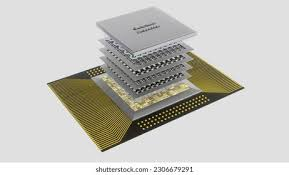
\includegraphics[width=0.45\textwidth]{image1.jpeg}
\caption{Superconducting qubits setup in a quantum computer}
\label{fig:superconducting}
\end{figure}

\subsection{Trapped Ions}
Trapped ion systems provide a high degree of control and precision, making them a strong candidate for scalable quantum computing. Research in this area focuses on improving coherence times and gate fidelities.

\begin{figure}[h]
\centering
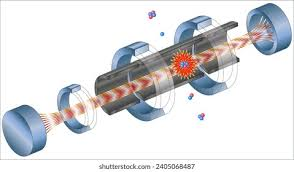
\includegraphics[width=0.45\textwidth]{image2.jpeg}
\caption{Trapped ions used in quantum computing experiments}
\label{fig:trapped_ions}
\end{figure}

\section{Quantum Applications}
Quantum computing has the potential to revolutionize various industries, from pharmaceuticals to finance. Key applications include optimization problems, quantum simulations, and secure communication.

\subsection{Optimization Problems}
Quantum algorithms can provide significant speedups for optimization problems, which are crucial in fields like logistics, finance, and artificial intelligence. For example, the Quantum Approximate Optimization Algorithm (QAOA) is used for combinatorial optimization:

\begin{equation}
    U(C, \gamma) = e^{-i \gamma C}
\end{equation}

\subsection{Quantum Simulations}
Quantum simulations of molecular and material properties can lead to breakthroughs in chemistry and material science, enabling the design of new drugs and materials. The Hamiltonian of a system is often simulated using:

\begin{equation}
    H = \sum_{i} c_i P_i
\end{equation}

\section{Challenges and Future Directions}
Despite the rapid advancements, several challenges remain in the field of quantum computing, including error correction, scalability, and the development of robust quantum software. Future research will likely focus on addressing these challenges and exploring new quantum algorithms and applications.

\section*{Acknowledgment}
The authors thank Quantum University and Tech Innovations Ltd for their support and collaboration in this research.

\section{Appendix}

\begin{table}[h]
\caption{Comparison of Quantum Algorithms}
\label{tab:algorithms}
\centering
\begin{tabular}{|c|c|c|}
\hline
\textbf{Algorithm} & \textbf{Problem Type} & \textbf{Speedup} \\
\hline
Shor's Algorithm & Factoring Integers & Exponential \\
\hline
Grover's Algorithm & Unsorted Database Search & Quadratic \\
\hline
QAOA & Combinatorial Optimization & Polynomial \\
\hline
VQE & Quantum Simulations & Exponential \\
\hline
\end{tabular}
\end{table}

\begin{thebibliography}{1}

\bibitem{Shor1994}
P. W. Shor, ``Algorithms for quantum computation: Discrete logarithms and factoring,'' in \emph{Proceedings of the 35th Annual Symposium on Foundations of Computer Science}, 1994, pp. 124-134.

\bibitem{Grover1996}
L. K. Grover, ``A fast quantum mechanical algorithm for database search,'' in \emph{Proceedings of the 28th Annual ACM Symposium on Theory of Computing}, 1996, pp. 212-219.

\bibitem{Nielsen2010}
M. A. Nielsen and I. L. Chuang, \emph{Quantum Computation and Quantum Information}, 10th Anniversary Edition, Cambridge University Press, 2010.

\end{thebibliography}

\end{document}
'